

%\killtitle % Removes the title 

%\cleardoublepage\newpage\thispagestyle{empty}\null
%\cleardoublepage\newpage\thispagestyle{empty}\null
%\cleardoublepage\newpage
\thispagestyle{empty}
%\begin{center}
%\includegraphics{images/dedication.pdf}
%\end{center}

\makebox[\textwidth]{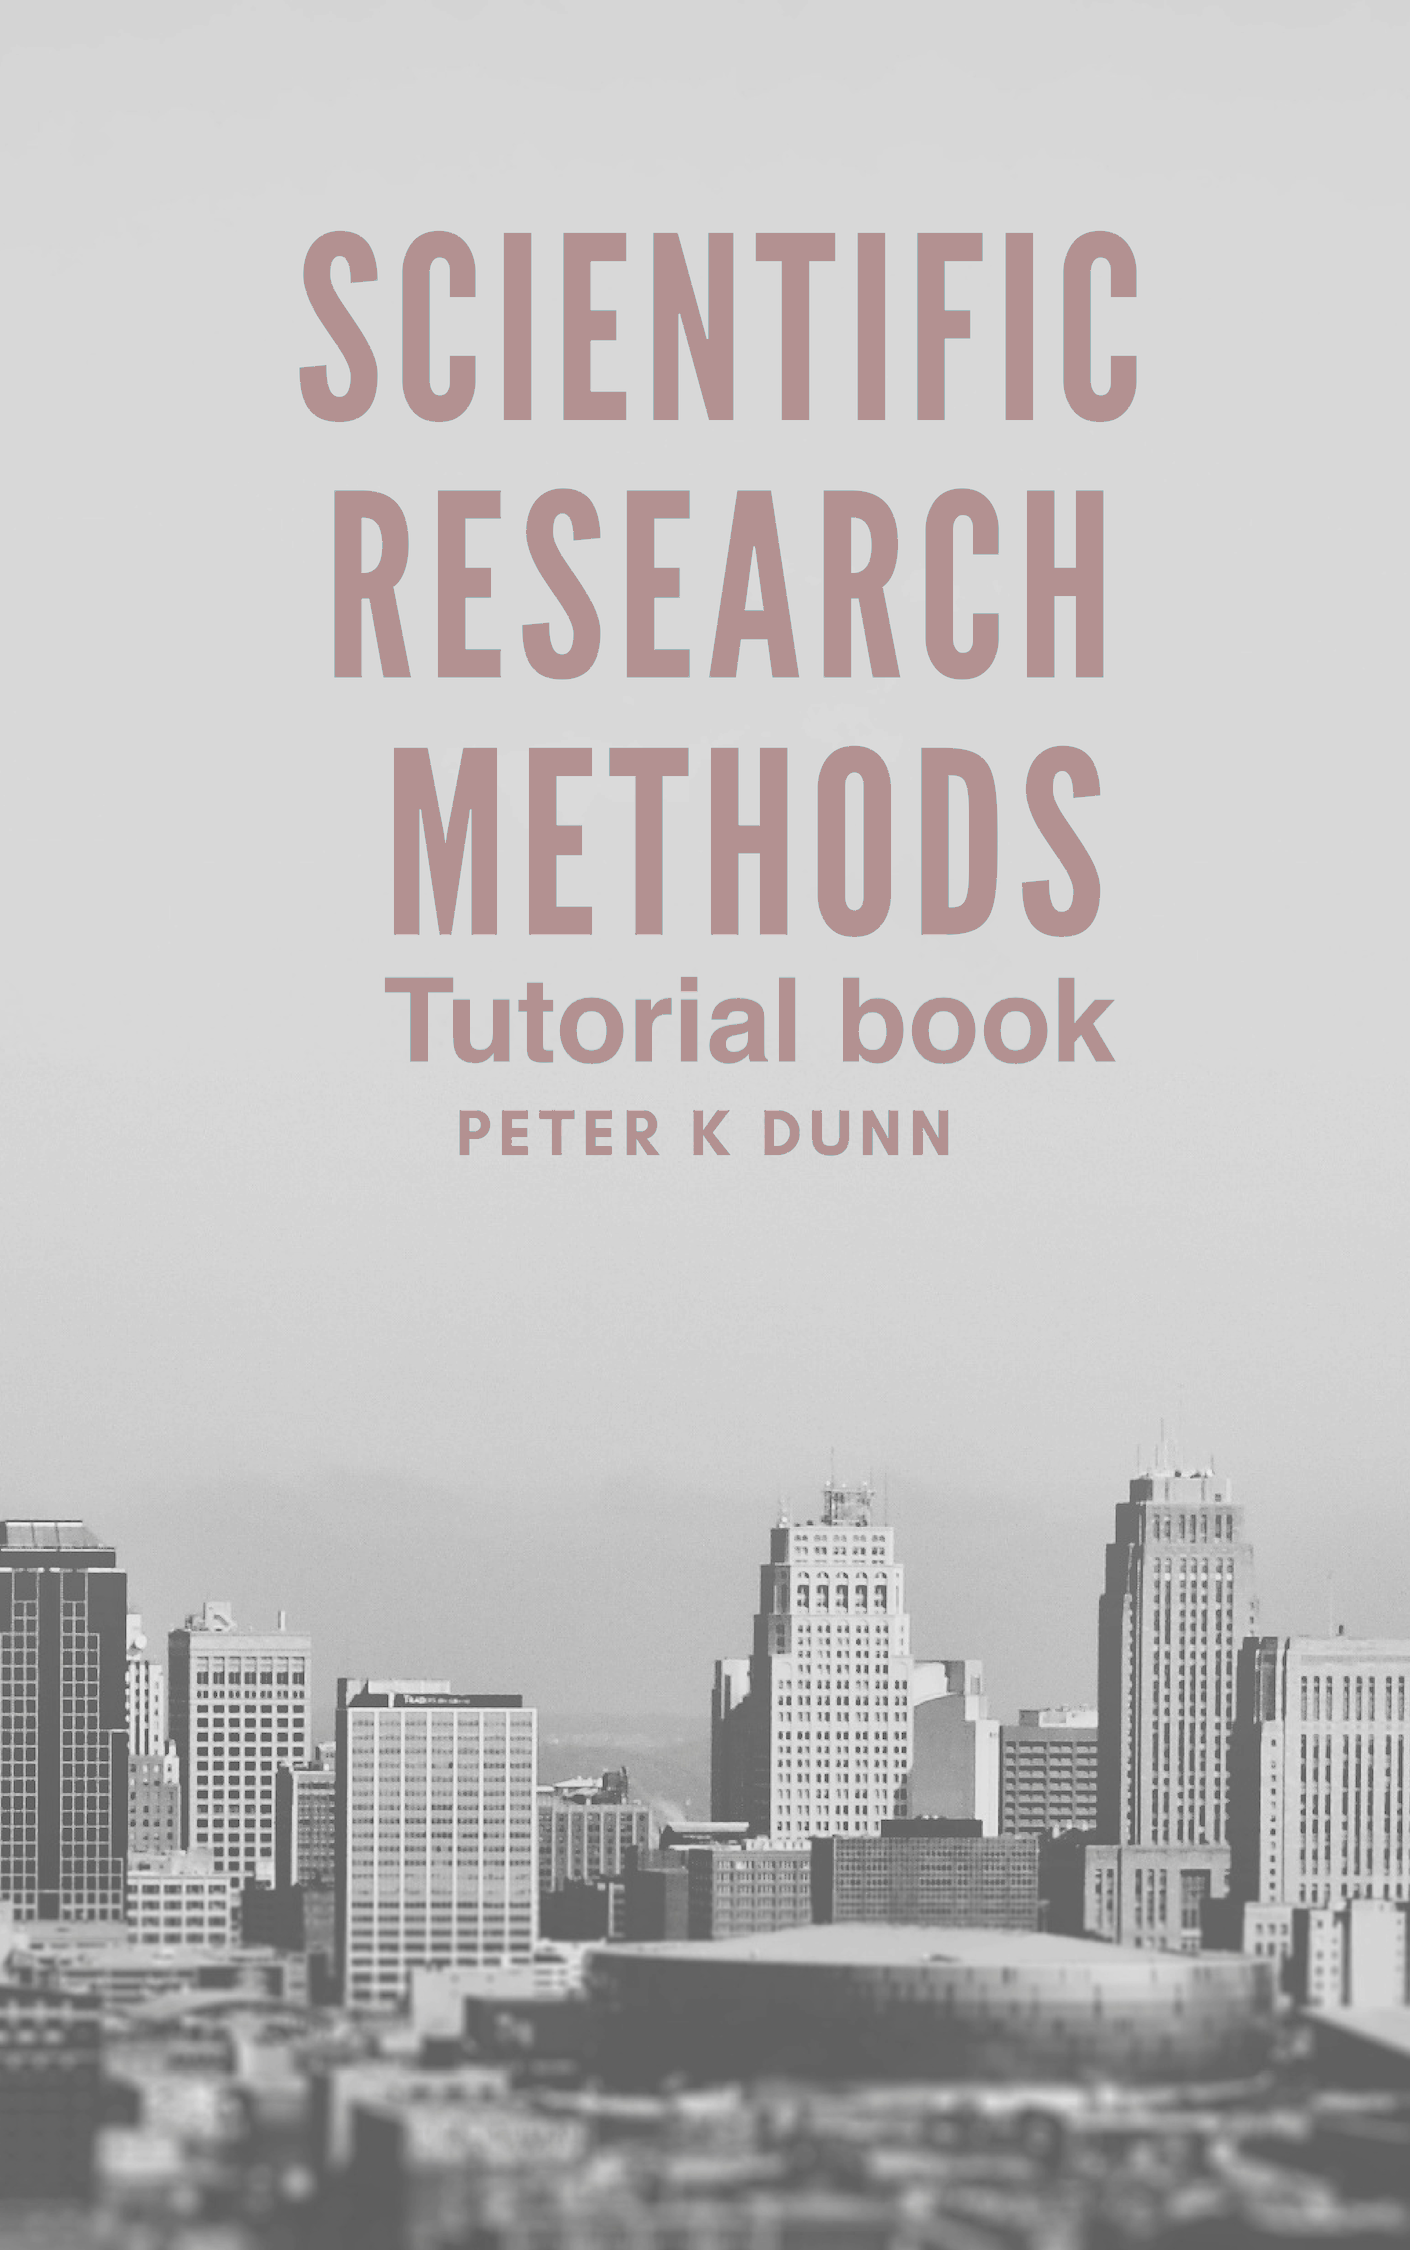
\includegraphics[width=\paperwidth]{images/cover-Tutorial.png}}
%\centerline{\includegraphics[width=\textwidth,height=\textheight]{images/cover.png}}

% Reinstate maketitle (https://stackoverflow.com/questions/45963505/coverpage-and-copyright-notice-before-title-in-r-bookdown):
\let\maketitle\oldmaketitle
\maketitle


\setlength{\abovedisplayskip}{-5pt}
\setlength{\abovedisplayshortskip}{-5pt}

%%% Footer
%\pagestyle{fancy}
%\fancyfoot[L]{\textit{Scientific Research Methods}}


%%% REDEFINE some environments

%%% BASED ONL
%%%   https://stackoverflow.com/questions/58195679/how-can-i-redefine-a-standard-bookdown-theorem-environment-in-latex-pdf (I asked)
%% and adapted using:
%%%   https://stackoverflow.com/questions/1565988/making-a-small-modification-to-a-latex-environment







\let\origexample=\example
\def\example{\begingroup\begin{quote}\setlength{\parskip}{3mm}\vspace{-7mm}\origexample}  
   %% -7mm removes some spacing at the top, which looked odd. Chosen by trial and error
   %% parskip added, otherwise no gap between paras in examples which looked odd.
\let\origendexample=\endexample
\def\endexample{\origendexample\end{quote}\endgroup}


\let\origdefinition=\definition
\def\definition{\begingroup\begin{quote}\vspace{-5mm}\origdefinition}  
   %% -5mm removes some spacing at the top, which looked odd. Chosen by trial and error
\let\origenddefinition=\enddefinition
\def\enddefinition{\origenddefinition\end{quote}\endgroup}


% \let\origlemma=\lemma
% \def\lemma{\begingroup\begin{quote}\vspace{-5mm}\origlemma\normalfont}  
%    %% -5mm removes some spacing at the top, which looked odd. Chosen by trial and error
% \let\origendlemma=\endlemma
% \def\endlemma{\origendlemma\end{quote}\endgroup}
% \renewenvironment{lemma}
%    {\begin{rmdthink}}
%    {\end{rmdthink}}







%%% Greyed background for lemma (now called Think)
% This works, but of course looses all the "lemma" stuff, like numbering and corss-referencing
%\renewenvironment{lemma}
%    {\begin{quote}}
%    {\end{quote}}


% Fix the itemize/enumerate spacing in exercises:
\let\origexercise=\exercise
\def\exercise{\begingroup\setitemize{labelindent=1.5em,labelsep=3mm,leftmargin=*}\setenumerate{labelindent=1.5em,labelsep=3mm,leftmargin=*}\origexercise}  
   %% -5mm removes some spacing at the top, which looked odd. Chosen by trial and error
\let\origendexercise=\endexercise
\def\endexercise{\origendexercise\endgroup}
   %% \setitem  from the  enumitem  package




% Exercise environment does not do dot points correctly: It does this:
%
%   1. This is the
%   way they are done.
%   No hanging pars
%
% So make some adjustments... but it is when itemize is called.


%\renewenvironment{example}[1]%
%  {\begin{quote}\textbf{#1:}}
%  {\end{quote}}